\pgfplotsset{compat=1.15}
\usetikzlibrary{arrows}
\definecolor{qqffqq}{rgb}{0,1,0}
\definecolor{qqqqff}{rgb}{0,0,1}
\definecolor{ffqqqq}{rgb}{1,0,0}
\definecolor{bfffqq}{rgb}{0.7490196078431373,1,0}
\definecolor{ffxfqq}{rgb}{1,0.4980392156862745,0}
\definecolor{qqffqq}{rgb}{0,1,0}
\definecolor{qqqqff}{rgb}{0,0,1}
\definecolor{ffqqqq}{rgb}{1,0,0}


\begin{figure}
	\centering
%	\caption{Problem data of the \SPPN, \TSPHN \ and \TSPN}
	\begin{minipage}{.3\textwidth}
		\caption{\SPPN \ instance}\label{fig:spp}
		\centering
		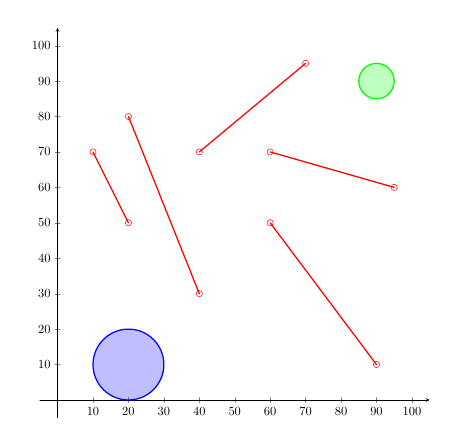
\begin{tikzpicture}[line cap=round,line join=round,>=triangle 45,x=1cm,y=1cm,scale=0.45]
		\begin{axis}[
		x=0.1cm,y=0.1cm,
		axis lines=middle,
		%ymajorgrids=true,
		%xmajorgrids=true,
		xmin=-5,
		xmax=105,
		ymin=-5,
		ymax=105,
		xtick={-30,-20,...,150},
		ytick={-20,-10,...,110},]
		\clip(-30.53772939574263,-29.679586779798747) rectangle (159.53639158056973,116.68410916363342);
		\draw [line width=1pt,color=ffqqqq] (20,80)-- (40,30);
		\draw [line width=1pt,color=ffqqqq] (70,95)-- (40,70);
		\draw [line width=1pt,color=ffqqqq] (95,60)-- (60,70);
		\draw [line width=1pt,color=ffqqqq] (60,50)-- (90,10);
		\draw [line width=1pt,color=ffqqqq] (10,70)-- (20,50);
		\draw [rotate around={0:(20,10)},line width=1pt,color=qqqqff,fill=qqqqff,fill opacity=0.25] (20,10) ellipse (1cm and 1cm);
		\draw [rotate around={0:(90,90)},line width=1pt,color=qqffqq,fill=qqffqq,fill opacity=0.25] (90,90) ellipse (0.5cm and 0.5cm);
		\begin{scriptsize}
		\draw [color=ffqqqq] (20,80) circle (2.5pt);
		\draw [color=ffqqqq] (40,30) circle (2.5pt);
		\draw [color=ffqqqq] (70,95) circle (2.5pt);
		\draw [color=ffqqqq] (40,70) circle (2.5pt);
		\draw [color=ffqqqq] (95,60) circle (2.5pt);
		\draw [color=ffqqqq] (60,70) circle (2.5pt);
		\draw [color=ffqqqq] (60,50) circle (2.5pt);
		\draw [color=ffqqqq] (90,10) circle (2.5pt);
		\draw [color=ffqqqq] (10,70) circle (2.5pt);
		\draw [color=ffqqqq] (20,50) circle (2.5pt);
		\end{scriptsize}
		\end{axis}
		\end{tikzpicture}
	\end{minipage}
	\hspace{0.2 in}
	\begin{minipage}{.3\textwidth}
		\caption{\TSPHN \ instance}\label{fig:tsph}
		\centering
		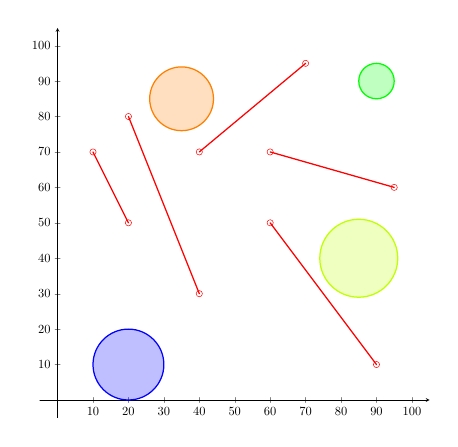
\begin{tikzpicture}[line cap=round,line join=round,>=triangle 45,x=1cm,y=1cm,scale=0.45]
		\begin{axis}[
		x=0.1cm,y=0.1cm,
		axis lines=middle,
		%ymajorgrids=true,
		%xmajorgrids=true,
		xmin=-5,
		xmax=105,
		ymin=-5,
		ymax=105,
		xtick={-30,-20,...,150},
		ytick={-20,-10,...,110},]
		\clip(-30.53772939574263,-29.679586779798747) rectangle (159.53639158056973,116.68410916363342);
		\draw [line width=1pt,color=ffqqqq] (20,80)-- (40,30);
		\draw [line width=1pt,color=ffqqqq] (70,95)-- (40,70);
		\draw [line width=1pt,color=ffqqqq] (95,60)-- (60,70);
		\draw [line width=1pt,color=ffqqqq] (60,50)-- (90,10);
		\draw [line width=1pt,color=ffqqqq] (10,70)-- (20,50);
		\draw [rotate around={0:(20,10)},line width=1pt,color=qqqqff,fill=qqqqff,fill opacity=0.25] (20,10) ellipse (1cm and 1cm);
		\draw [rotate around={0:(90,90)},line width=1pt,color=qqffqq,fill=qqffqq,fill opacity=0.25] (90,90) ellipse (0.5cm and 0.5cm);
		\draw [rotate around={0:(35,85)},line width=1pt,color=ffxfqq,fill=ffxfqq,fill opacity=0.25] (35,85) ellipse (0.9cm and 0.9cm);
		\draw [rotate around={0:(85,40)},line width=1pt,color=bfffqq,fill=bfffqq,fill opacity=0.25] (85,40) ellipse (1.1cm and 1.1cm);
		\begin{scriptsize}
		\draw [color=ffqqqq] (20,80) circle (2.5pt);
		\draw [color=ffqqqq] (40,30) circle (2.5pt);
		\draw [color=ffqqqq] (70,95) circle (2.5pt);
		\draw [color=ffqqqq] (40,70) circle (2.5pt);
		\draw [color=ffqqqq] (95,60) circle (2.5pt);
		\draw [color=ffqqqq] (60,70) circle (2.5pt);
		\draw [color=ffqqqq] (60,50) circle (2.5pt);
		\draw [color=ffqqqq] (90,10) circle (2.5pt);
		\draw [color=ffqqqq] (10,70) circle (2.5pt);
		\draw [color=ffqqqq] (20,50) circle (2.5pt);
		\end{scriptsize}
		\end{axis}
		\end{tikzpicture}

	\end{minipage}
	\hspace{0.2 in}
	\begin{minipage}{.3\textwidth}
		\centering
		\caption{\TSPN \ instance}\label{fig:tsp}
		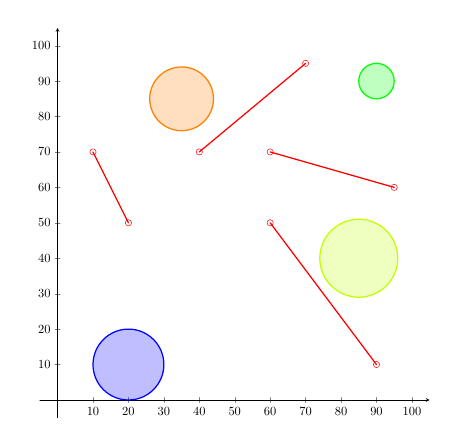
\begin{tikzpicture}[line cap=round,line join=round,>=triangle 45,x=1cm,y=1cm,scale=0.45]
			\begin{axis}[
				x=0.1cm,y=0.1cm,
				axis lines=middle,
				%ymajorgrids=true,
				%xmajorgrids=true,
				xmin=-5,
				xmax=105,
				ymin=-5,
				ymax=105,
				xtick={-30,-20,...,150},
				ytick={-20,-10,...,110},]
				\clip(-30.53772939574263,-29.679586779798747) rectangle (159.53639158056973,116.68410916363342);
				\draw [line width=1pt,color=ffqqqq] (70,95)-- (40,70);
				\draw [line width=1pt,color=ffqqqq] (95,60)-- (60,70);
				\draw [line width=1pt,color=ffqqqq] (60,50)-- (90,10);
				\draw [line width=1pt,color=ffqqqq] (10,70)-- (20,50);
				\draw [rotate around={0:(20,10)},line width=1pt,color=qqqqff,fill=qqqqff,fill opacity=0.25] (20,10) ellipse (1cm and 1cm);
				\draw [rotate around={0:(90,90)},line width=1pt,color=qqffqq,fill=qqffqq,fill opacity=0.25] (90,90) ellipse (0.5cm and 0.5cm);
				\draw [rotate around={0:(35,85)},line width=1pt,color=ffxfqq,fill=ffxfqq,fill opacity=0.25] (35,85) ellipse (0.9cm and 0.9cm);
				\draw [rotate around={0:(85,40)},line width=1pt,color=bfffqq,fill=bfffqq,fill opacity=0.25] (85,40) ellipse (1.1cm and 1.1cm);
				\begin{scriptsize}
					\draw [color=ffqqqq] (70,95) circle (2.5pt);
					\draw [color=ffqqqq] (40,70) circle (2.5pt);
					\draw [color=ffqqqq] (95,60) circle (2.5pt);
					\draw [color=ffqqqq] (60,70) circle (2.5pt);
					\draw [color=ffqqqq] (60,50) circle (2.5pt);
					\draw [color=ffqqqq] (90,10) circle (2.5pt);
					\draw [color=ffqqqq] (10,70) circle (2.5pt);
					\draw [color=ffqqqq] (20,50) circle (2.5pt);
				\end{scriptsize}
			\end{axis}
		\end{tikzpicture}
	\end{minipage}
	\label{fig:initialdata}
\end{figure}